\documentclass[aspectratio=169]{beamer}
%[handout]

\usetheme[progressbar=frametitle]{metropolis}
\usepackage{appendixnumberbeamer}

\usepackage[utf8]{inputenc}
\usepackage[T1]{fontenc}

\usepackage[brazil]{babel}
\usepackage[outputdir=..]{minted}
\usepackage{xcolor}
\usepackage{soul} % strikethrough
\usepackage{advdate}
\usepackage{graphicx}
\graphicspath{{figs/}}
\usepackage{graphbox}

\usepackage[ampersand]{easylist}

\usepackage{multirow}
\usepackage{multicol}
\usepackage{subcaption}

\usepackage{pgf,tikz}
\usetikzlibrary{shapes,arrows,positioning}
\usetikzlibrary{circuits.logic.US}
\usetikzlibrary{matrix,calc}

\usepackage{karnaugh-map}

\usepackage{pgfpages}
\setbeameroption{hide notes} % Only slides
% \setbeameroption{show only notes} % Only notes
% \setbeameroption{show notes on second screen=right} % Both

% \graphicspath{{../figs/}}

\definecolor{bgc}{rgb}{0.95,0.9,0.95}
\definecolor{links}{HTML}{2A7F7F}
\hypersetup{colorlinks,linkcolor=,urlcolor=links}

\newminted{verilog}{fontsize=\scriptsize, 
    linenos,
    numbersep=8pt,
    bgcolor=bgc,
    tabsize=4,
    framesep=3mm} 
    %frame=lines,

\newcommand{\verilog}[1]{\verilogf{#1}{\footnotesize}}

\newcommand{\verilogf}[2]{\inputminted[fontsize=#2, 
    linenos,
    tabsize=2,
    numbersep=4pt,
    bgcolor=bgc,
    framesep=3mm]{verilog}{../codes/#1.v}
}

\newminted{nasm}{fontsize=\scriptsize, 
		   linenos,
		   numbersep=8pt,
           bgcolor=bgc,
		   framesep=3mm} 

\usepackage{booktabs}
\usepackage[scale=2]{ccicons}

\usepackage{pgfplots}
\usepgfplotslibrary{dateplot}

\usepackage{hyperref}


\usepackage{xspace}
\newcommand{\themename}{\textbf{\textsc{metropolis}}\xspace}



\usepackage{pifont}% http://ctan.org/pkg/pifont
\newcommand{\cmark}{\ding{51}}%
\newcommand{\xmark}{\ding{55}}%

% \tiny	
% \scriptsize
% \footnotesize
% \small	
% \normalsize	
% \large	
% \Large	
% \LARGE	
% \huge	
% \Huge	



\newminted{python}{fontsize=\scriptsize, 
		   linenos,
		   breaklines,
		   numbersep=8pt,
           tabsize=2,
		   framesep=3mm} 
		   
\newminted{verilog}{fontsize=\scriptsize, 
		   linenos,
		   breaklines,
		   numbersep=8pt,
           tabsize=2,
		   framesep=3mm} 
		   




\definecolor{bgc}{rgb}{0.95,0.9,0.95}
\definecolor{links}{HTML}{2A7F7F}
\hypersetup{colorlinks,linkcolor=,urlcolor=links}


% \usepackage[style=apa]{biblatex}
% \addbibresource{mm.bib}


% \author{\large Prof. Ricardo Menotti (\href{mailto:menotti@ufscar.br}{menotti@ufscar.br})}

\newcommand{\newauthor}[2]{
  \parbox{0.50\textwidth}{
    \texorpdfstring
      {
        \centering
        \small #1 \newline
        {\scriptsize{\urlstyle{same}\href{mailto:#2}{#2}\urlstyle{tt}}}
      }
      {#1} \newline
  }
}

\author{
  \newauthor{Prof. Ricardo Menotti}{menotti@ufscar.br}
\and \newauthor{Prof. Luciano de Oliveira Neris}{lneris@ufscar.br}  
%\and \newauthor{Prof. Artino Quintino da Silva Filho}{artino@ufscar.br}
% \and \newauthor{Prof. Maurício Figueiredo}{mauricio@ufscar.br}
% \and \newauthor{Prof. Edilson Kato}{kato@ufscar.br}
% \and \newauthor{Prof. Roberto Inoue}{rsinoue@ufscar.br}
}

\date{Atualizado em: \today}

\institute{\large \textbf{Departamento de Computação} \\
Centro de Ciências Exatas e de Tecnologia \\
Universidade Federal de São Carlos}

\title{Lógica Digital (1001351)}

\titlegraphic{\hfill
\includegraphics[height=1.5cm]{LogoUfscar}}



\subtitle{Circuitos Sequenciais: Latches e Flip-flops} % 

\begin{document}

\begin{frame}
	\titlepage
\end{frame} 

\section{Circuitos Sequenciais}

\begin{frame}{Objetivos}   %\centering
    Nesta aula vamos aprender sobre:
    \begin{itemize}
        \item Circuitos lógicos que podem armazenar informações;
        \item Latches e Flip-flops, os quais armazenam um único bit.
    \end{itemize}
\end{frame}

\begin{frame}{Necessidade}   \centering
    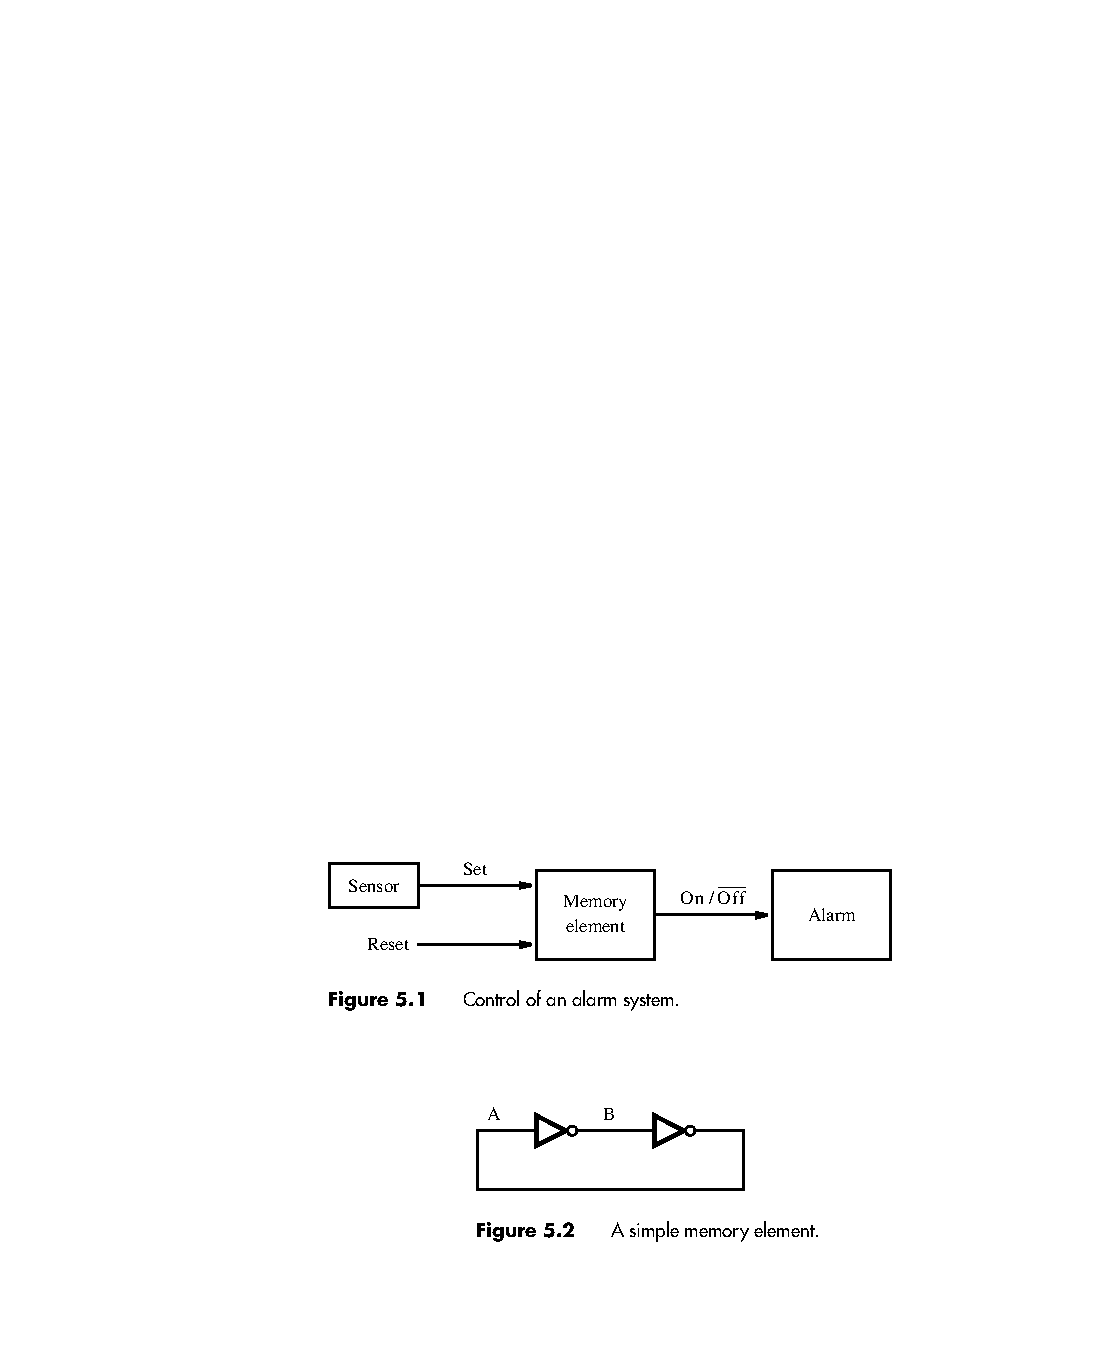
\includegraphics[width=.75\textwidth]{VerilogFig5_1_2} \\
\end{frame}

\begin{frame}{Latch básico}   \centering
    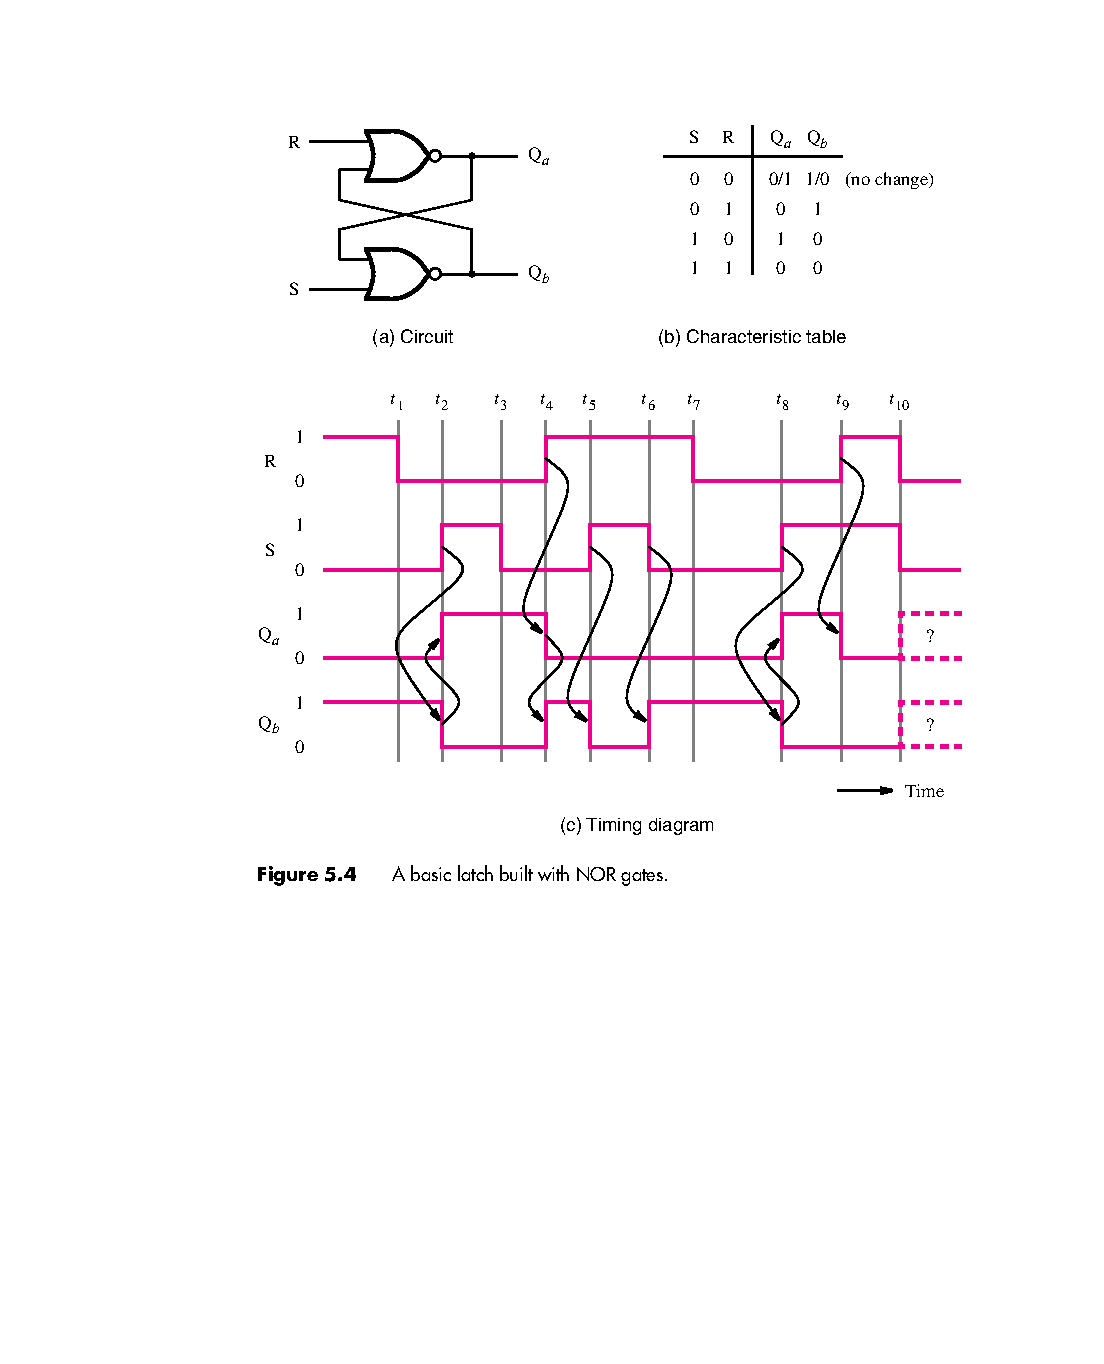
\includegraphics[width=.6\textwidth]{VerilogFig5_4} \\
\end{frame}

\begin{frame}{Latch com habilita \textit{(gated latch)}}   \centering
    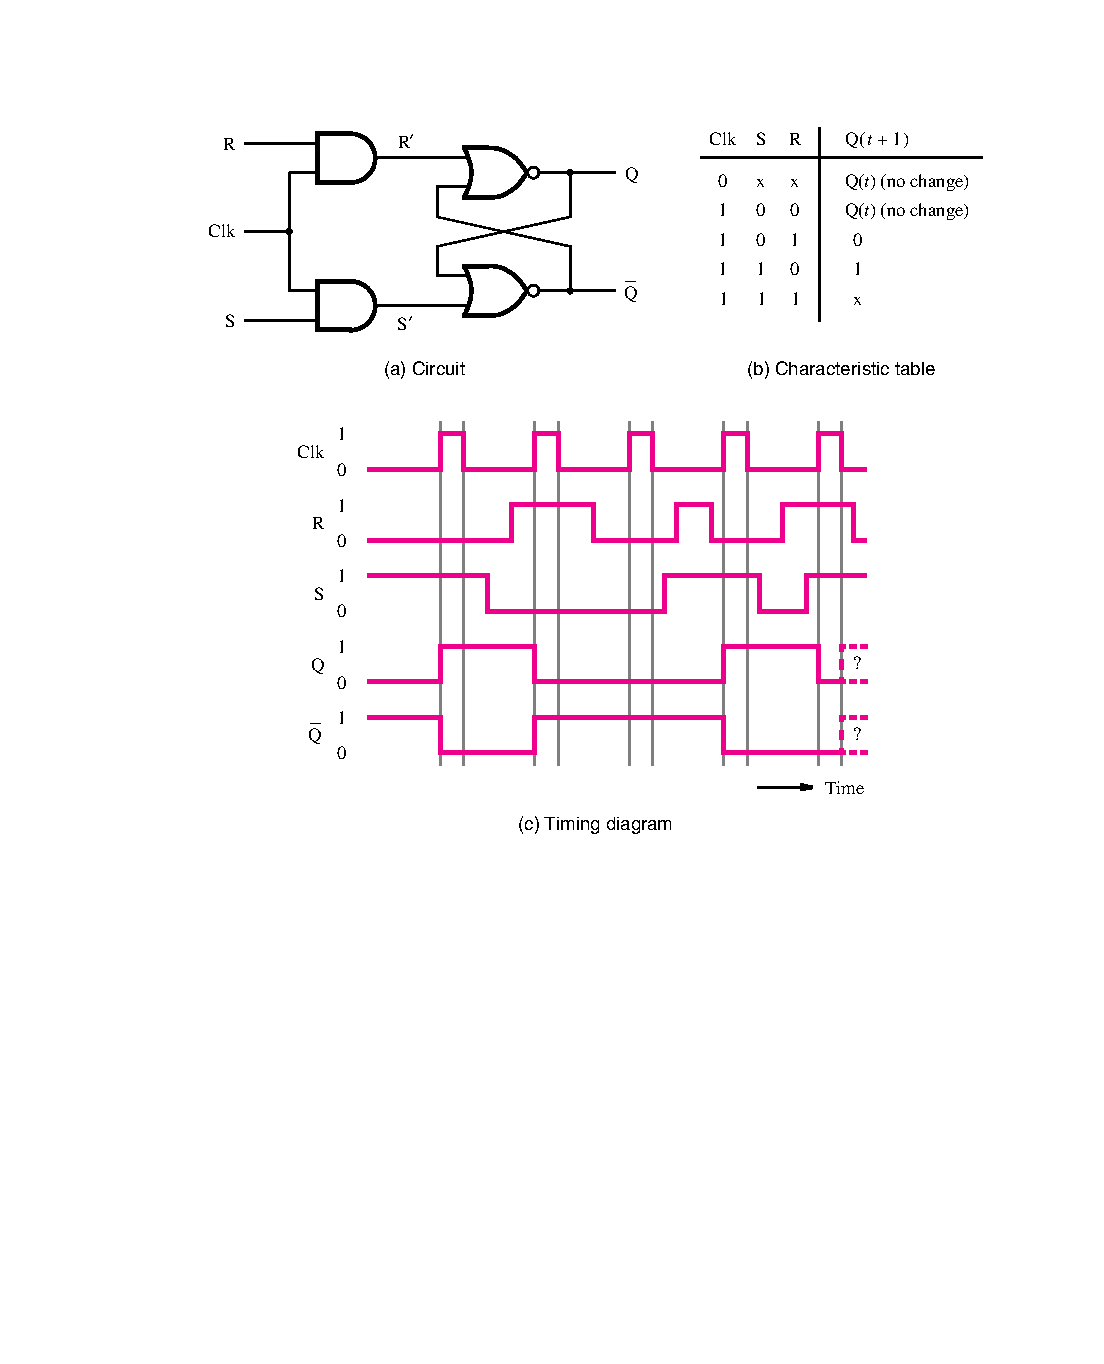
\includegraphics[width=.6\textwidth]{VerilogFig5_5abc} \\
\end{frame}

\begin{frame}{Latch com habilita \textit{(gated latch)}}   \centering
    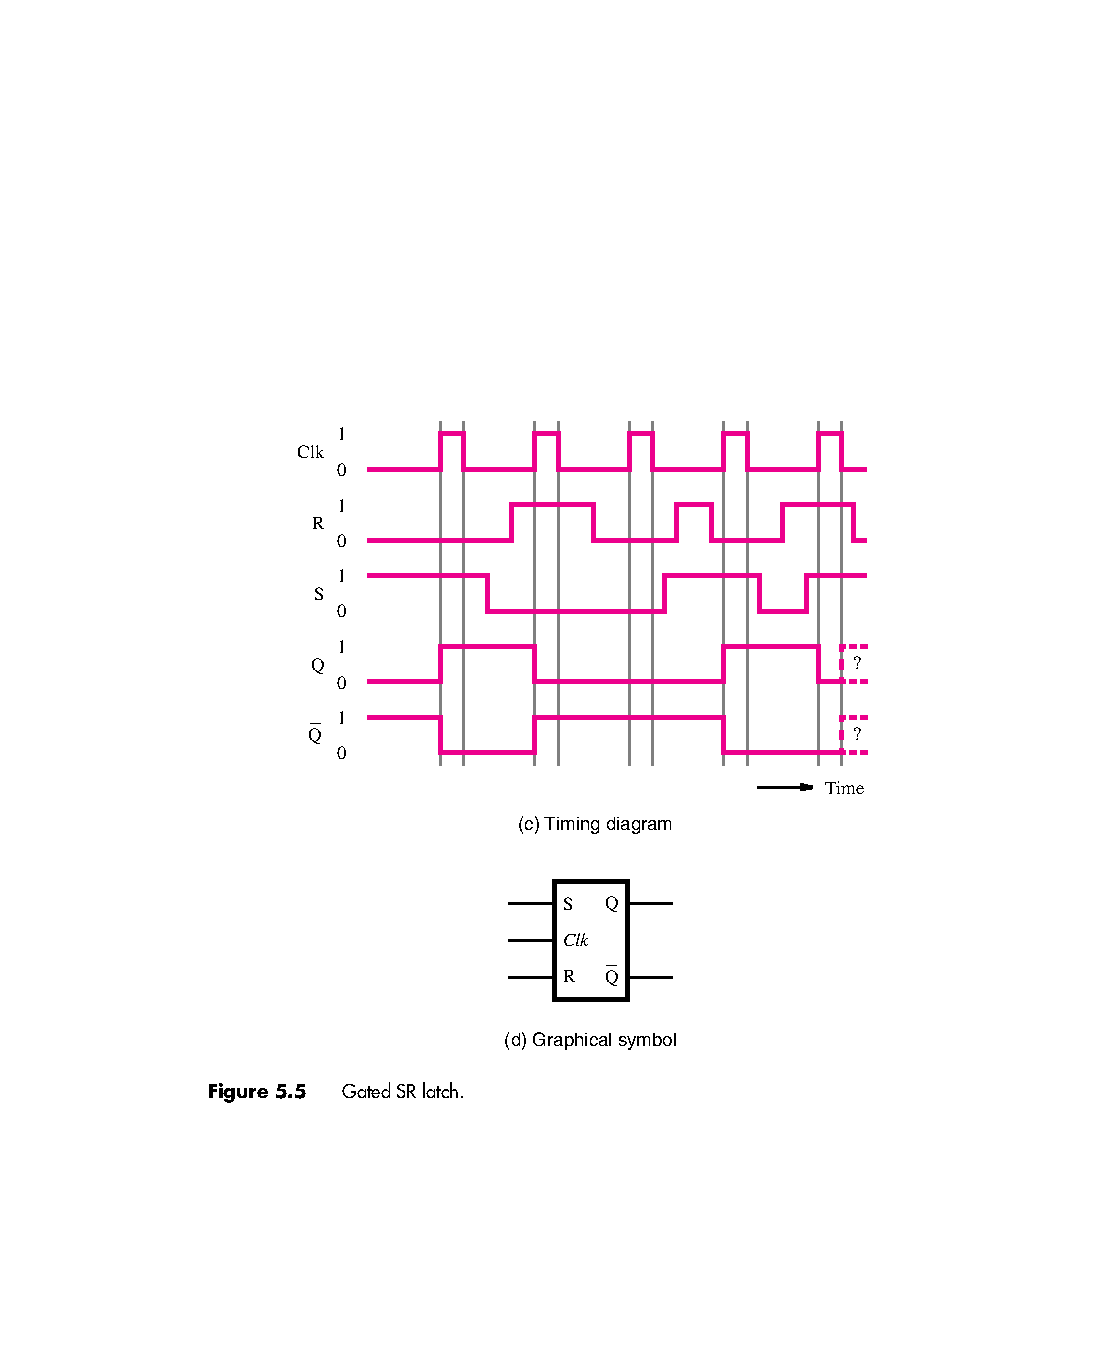
\includegraphics[width=.6\textwidth]{VerilogFig5_5cd} \\
\end{frame}

\begin{frame}{Latch construído com portas NAND}   \centering
    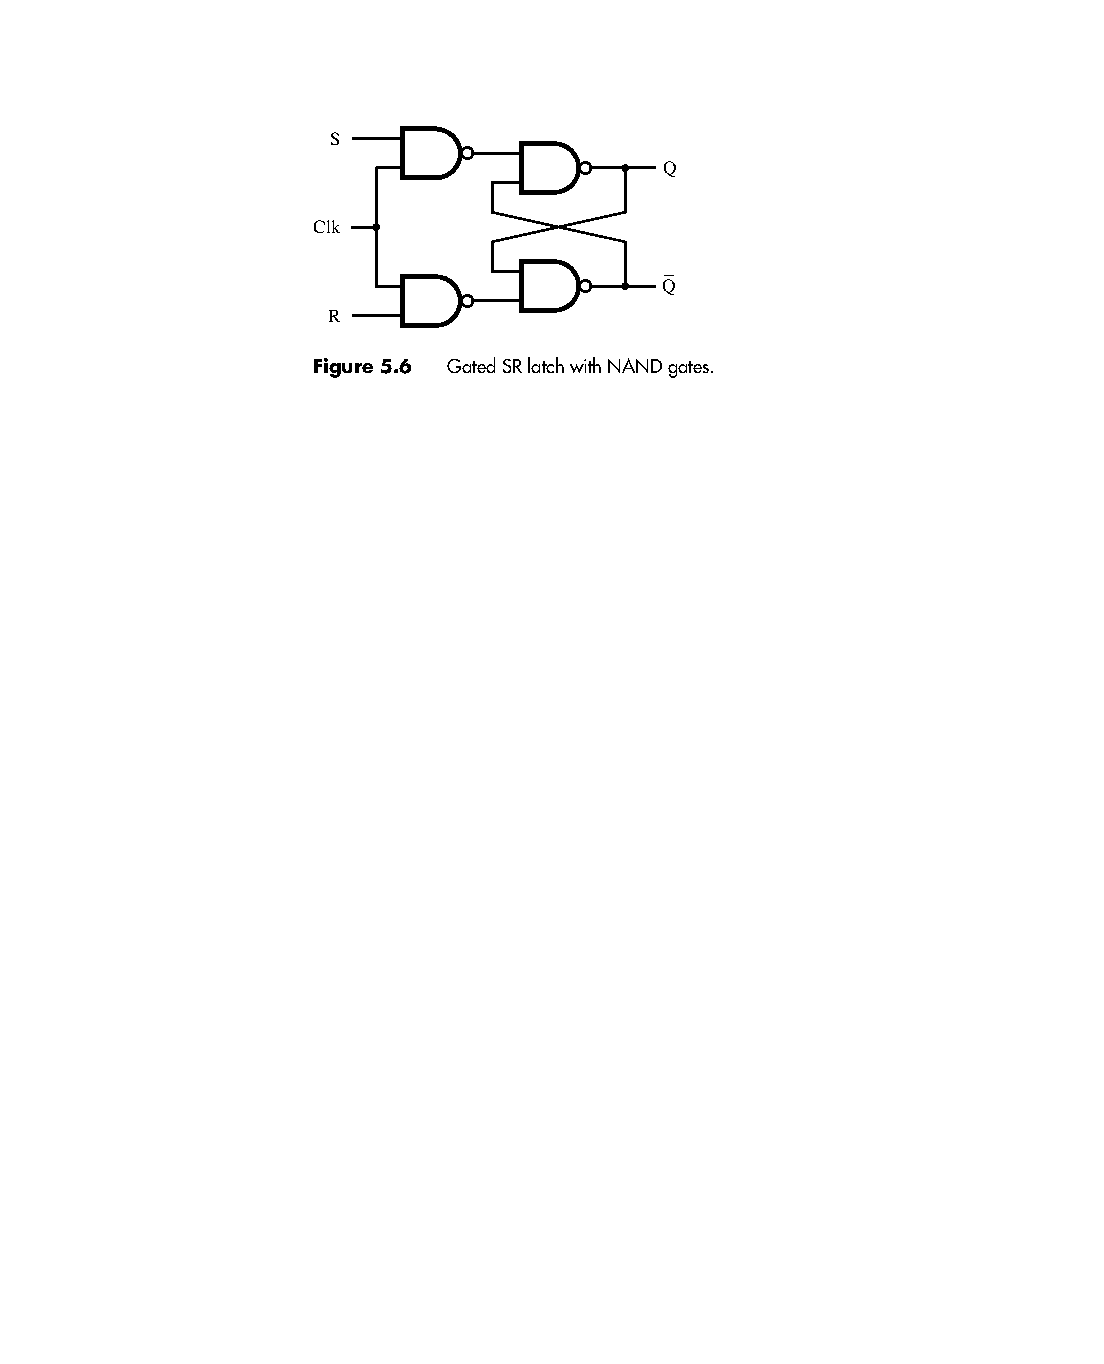
\includegraphics[width=.5\textwidth]{VerilogFig5_6} \\
\end{frame}

\begin{frame}{Latch D}   \centering
    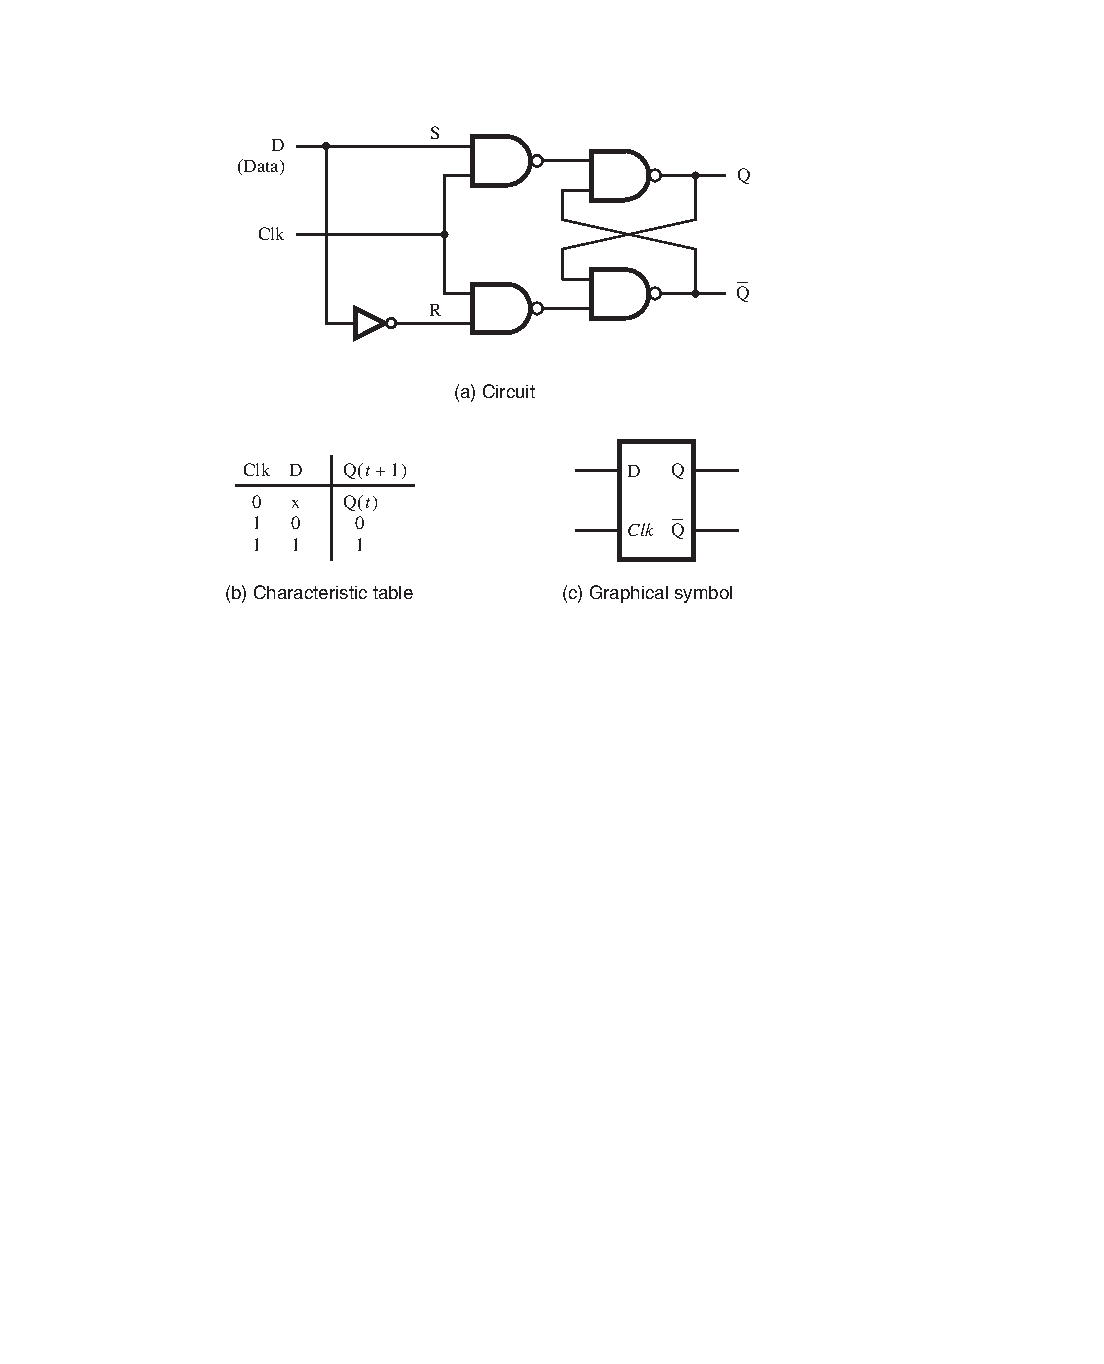
\includegraphics[width=.6\textwidth]{VerilogFig5_7abc} \\
\end{frame}

\begin{frame}{Latch D}   \centering
    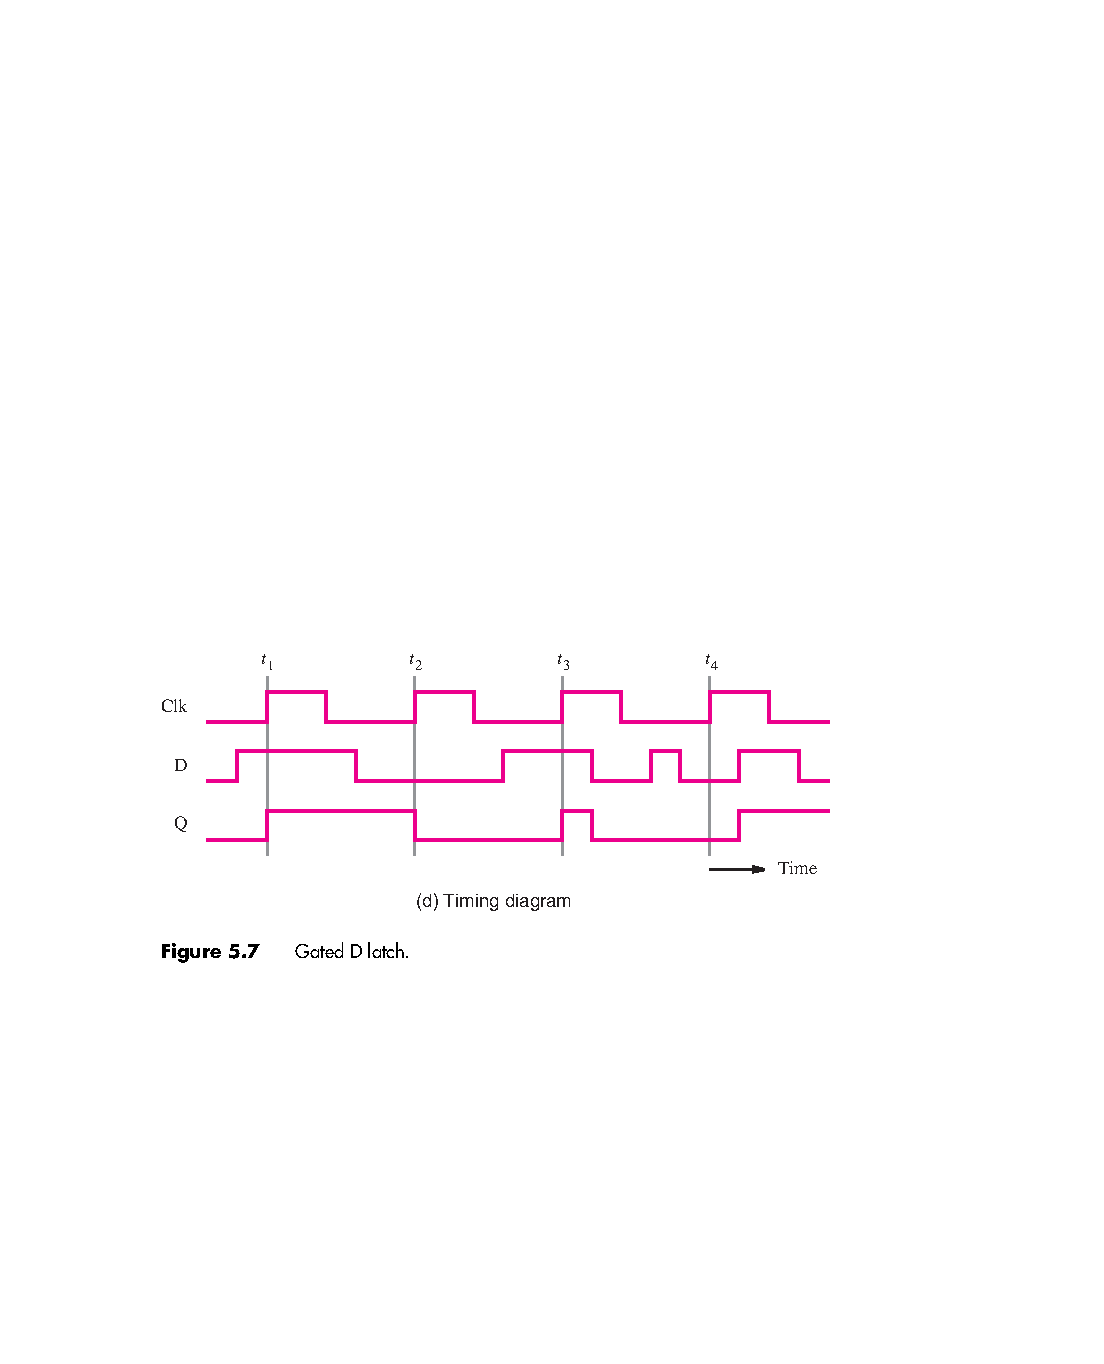
\includegraphics[width=\textwidth]{VerilogFig5_7d} \\
\end{frame}

\begin{frame}{Flip-flop D Mestre/Escravo}   \centering
    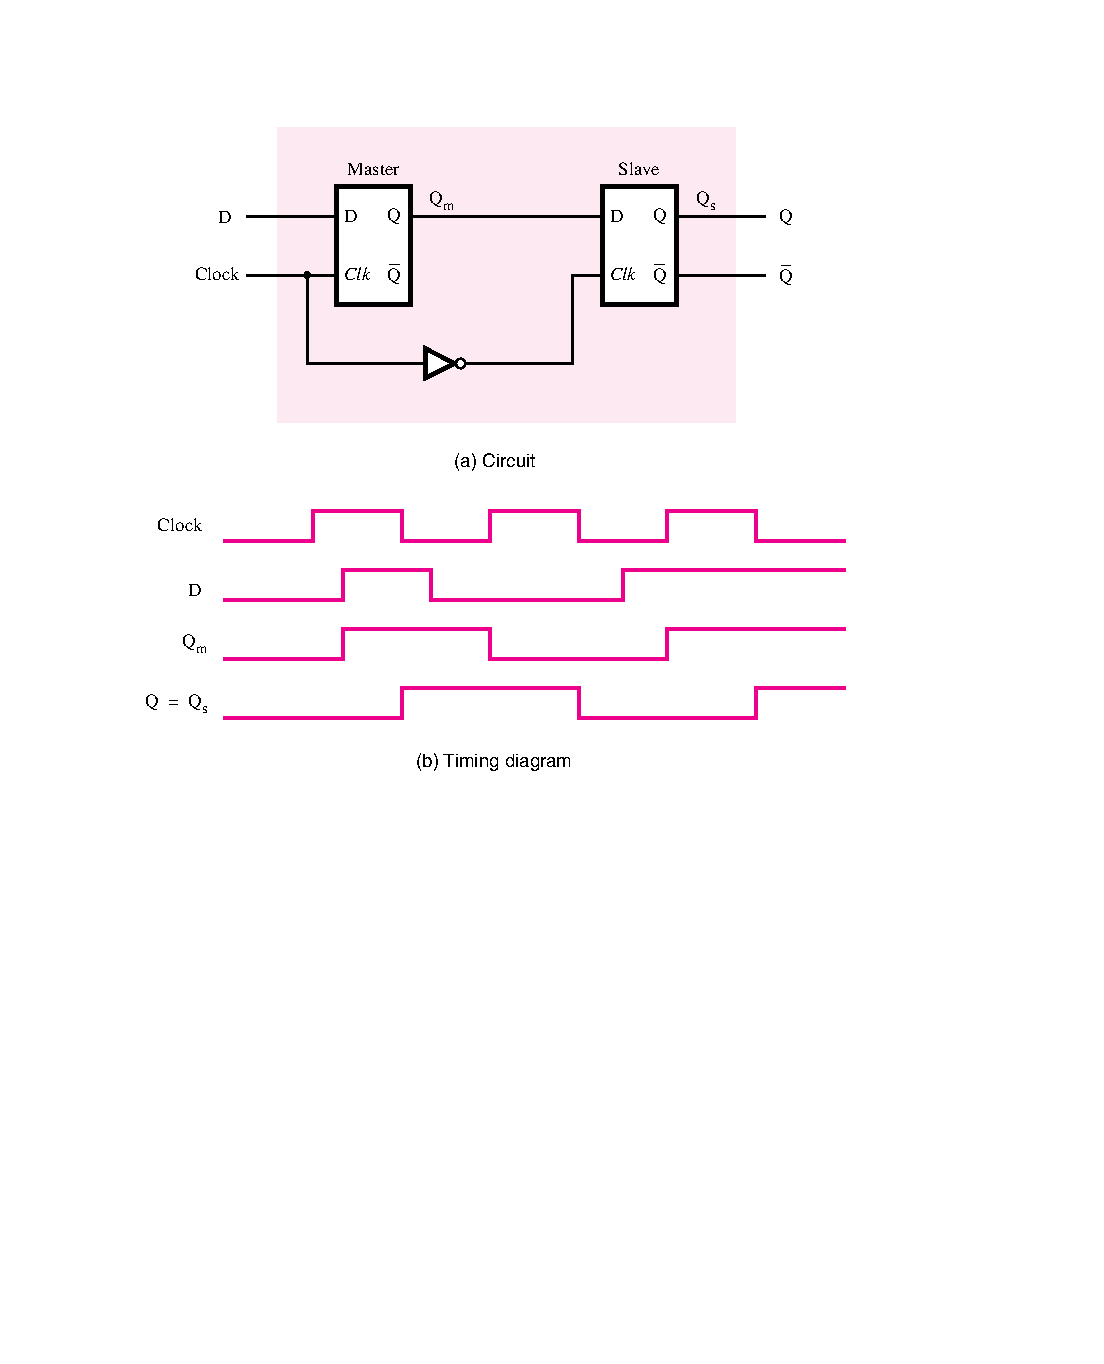
\includegraphics[width=.6\textwidth]{VerilogFig5_9ab} \\
\end{frame}

\begin{frame}{Flip-flop D Mestre/Escravo}   \centering
    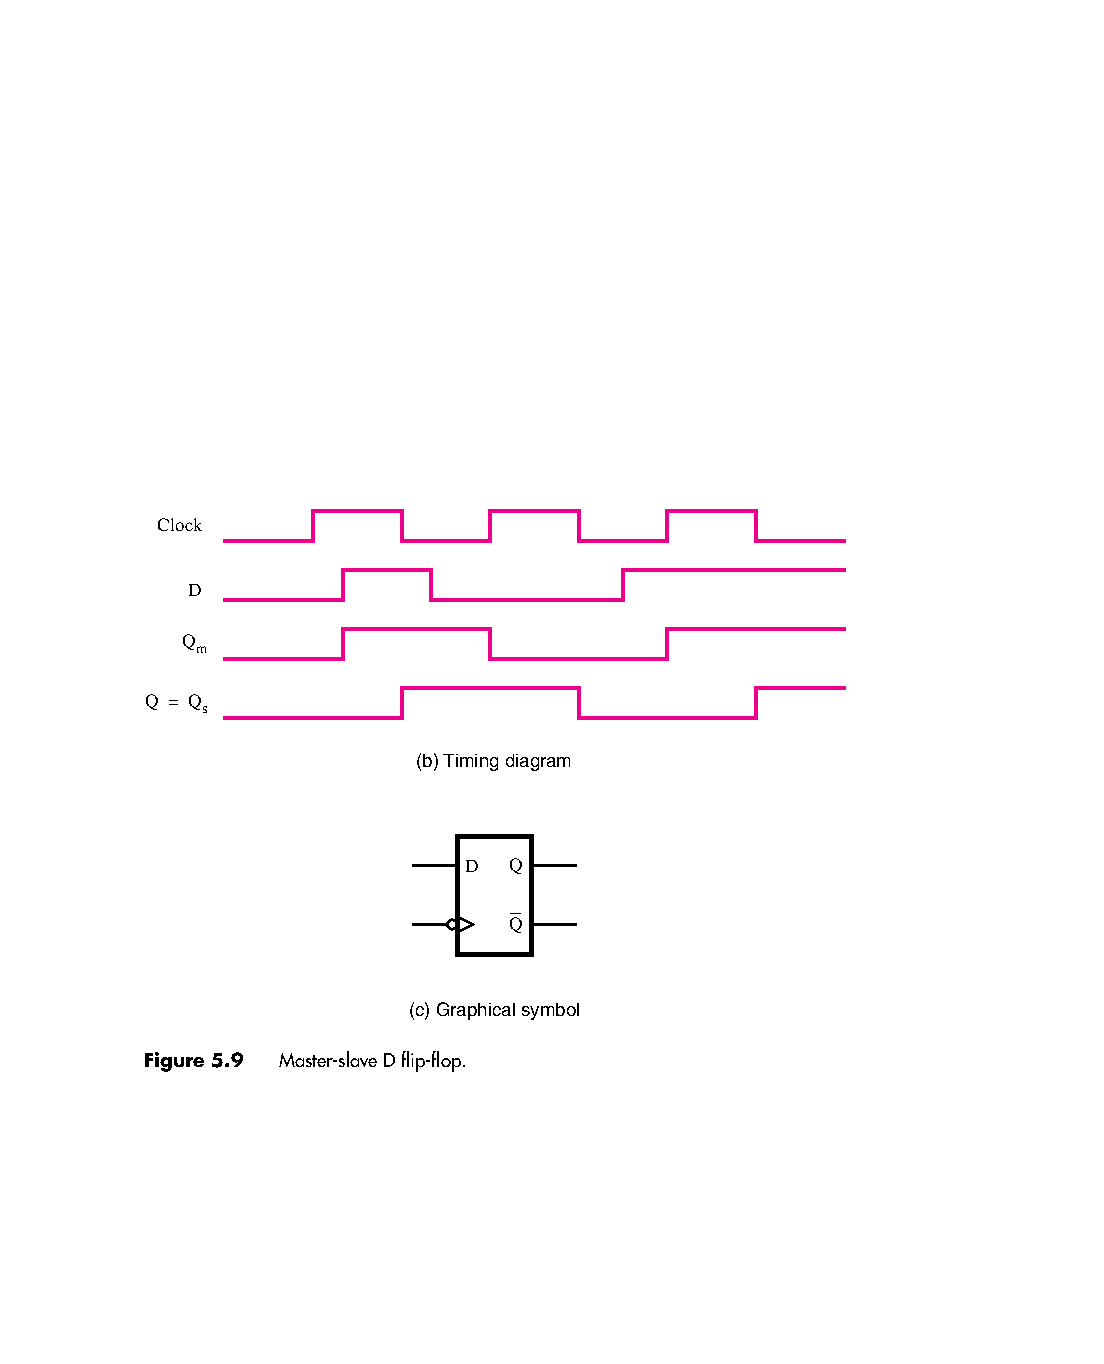
\includegraphics[width=.6\textwidth]{VerilogFig5_9bc} \\
\end{frame}

\begin{frame}{Flip-flop D com borda positiva (subida)}   \centering
    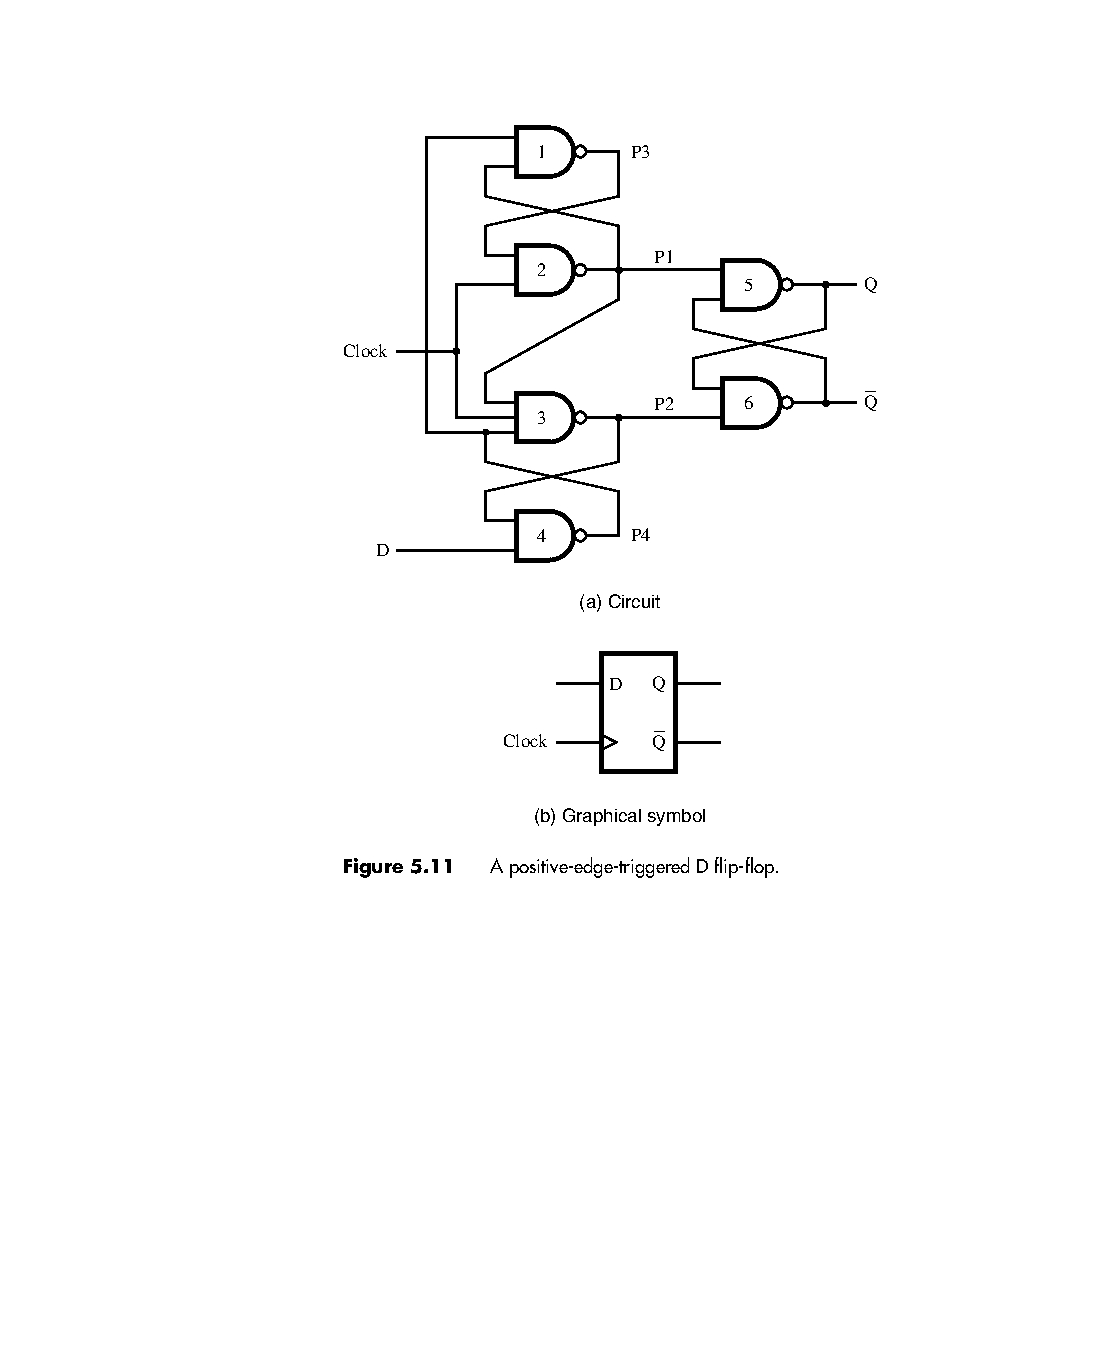
\includegraphics[width=.4\textwidth]{VerilogFig5_11} \\
\end{frame}

\begin{frame}{Flip-flop D Mestre/Escravo com Clear e Preset}   \centering
    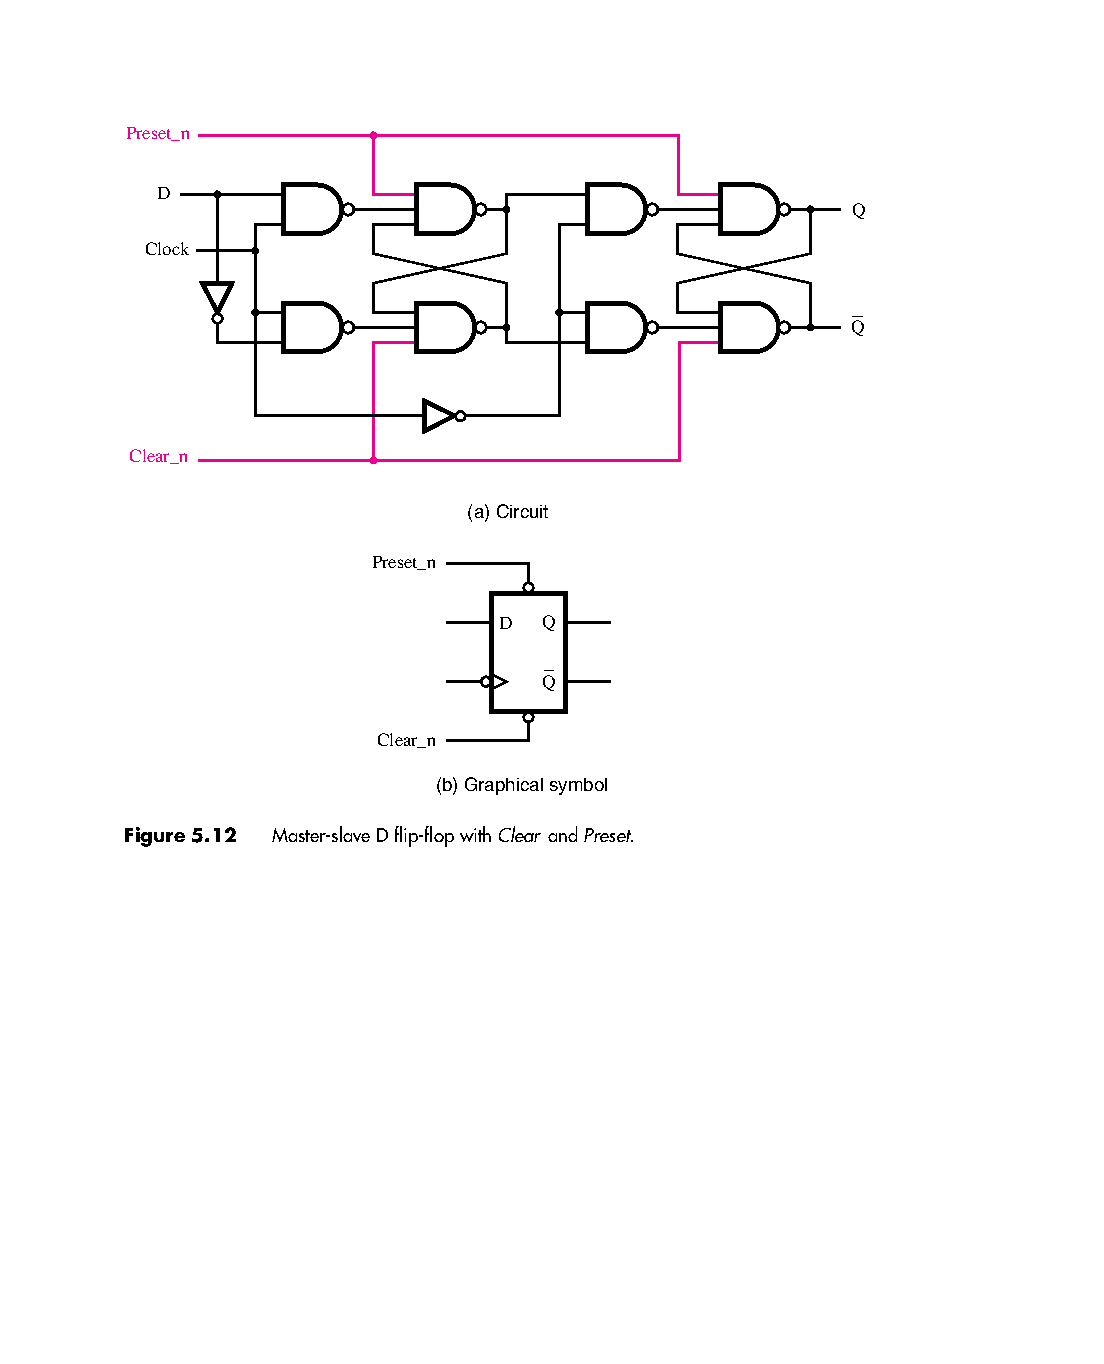
\includegraphics[width=.55\textwidth]{VerilogFig5_12} \\
\end{frame}

\begin{frame}{Flip-flop D Mestre/Escravo com borda positiva}   \centering
    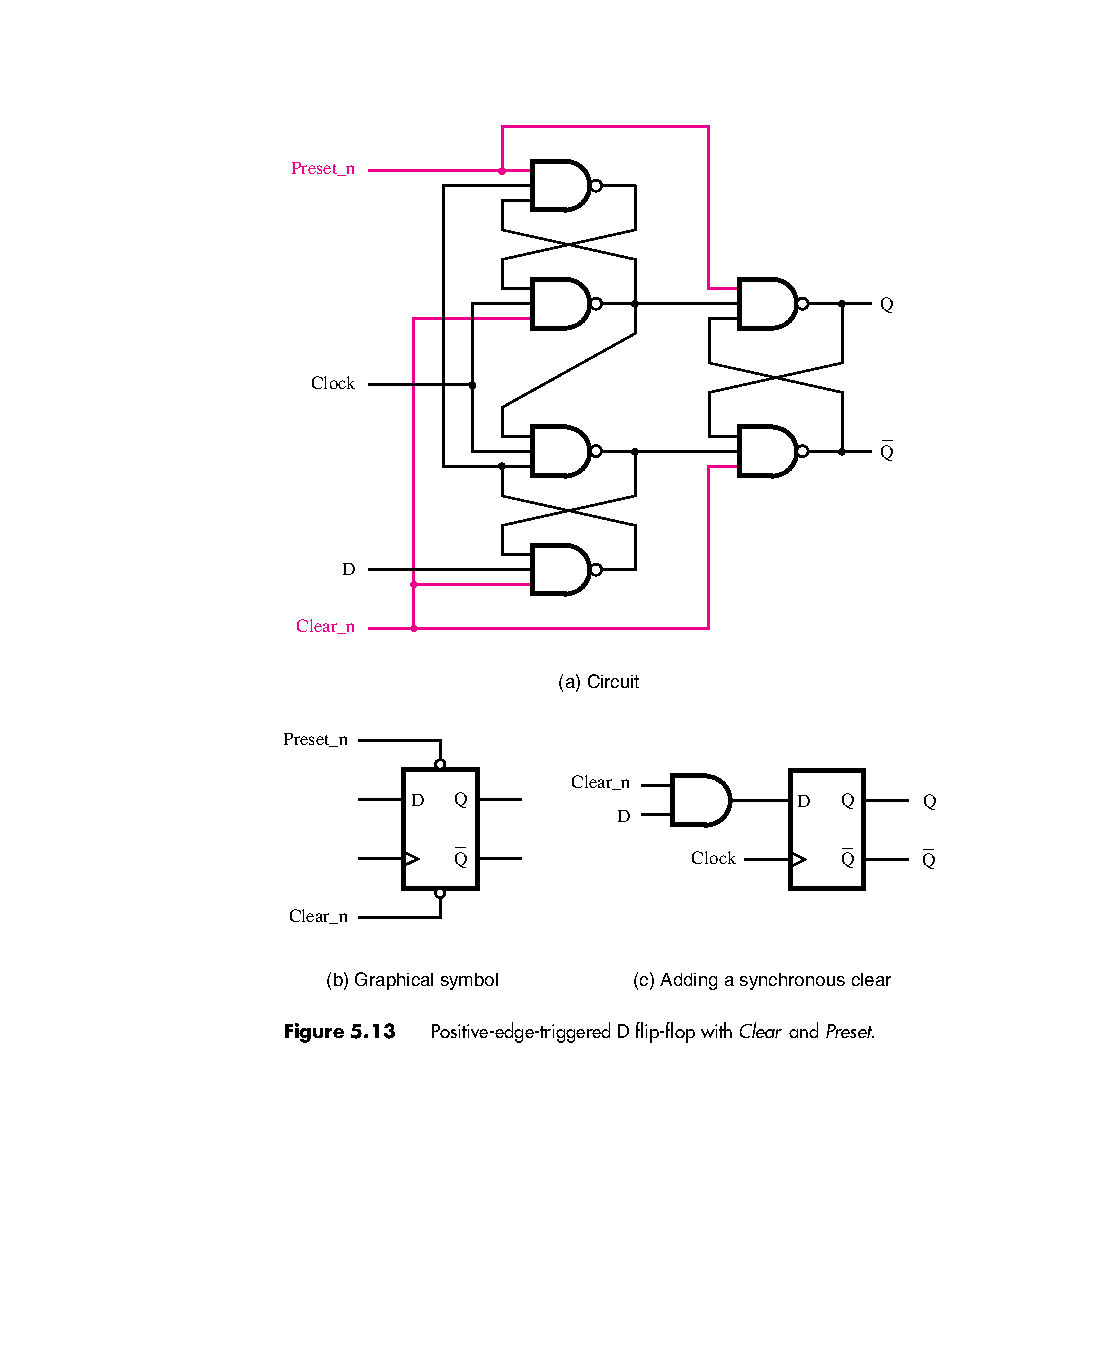
\includegraphics[width=.45\textwidth]{VerilogFig5_13} \\
\end{frame}

\begin{frame}{Flip-flop T}   \centering
    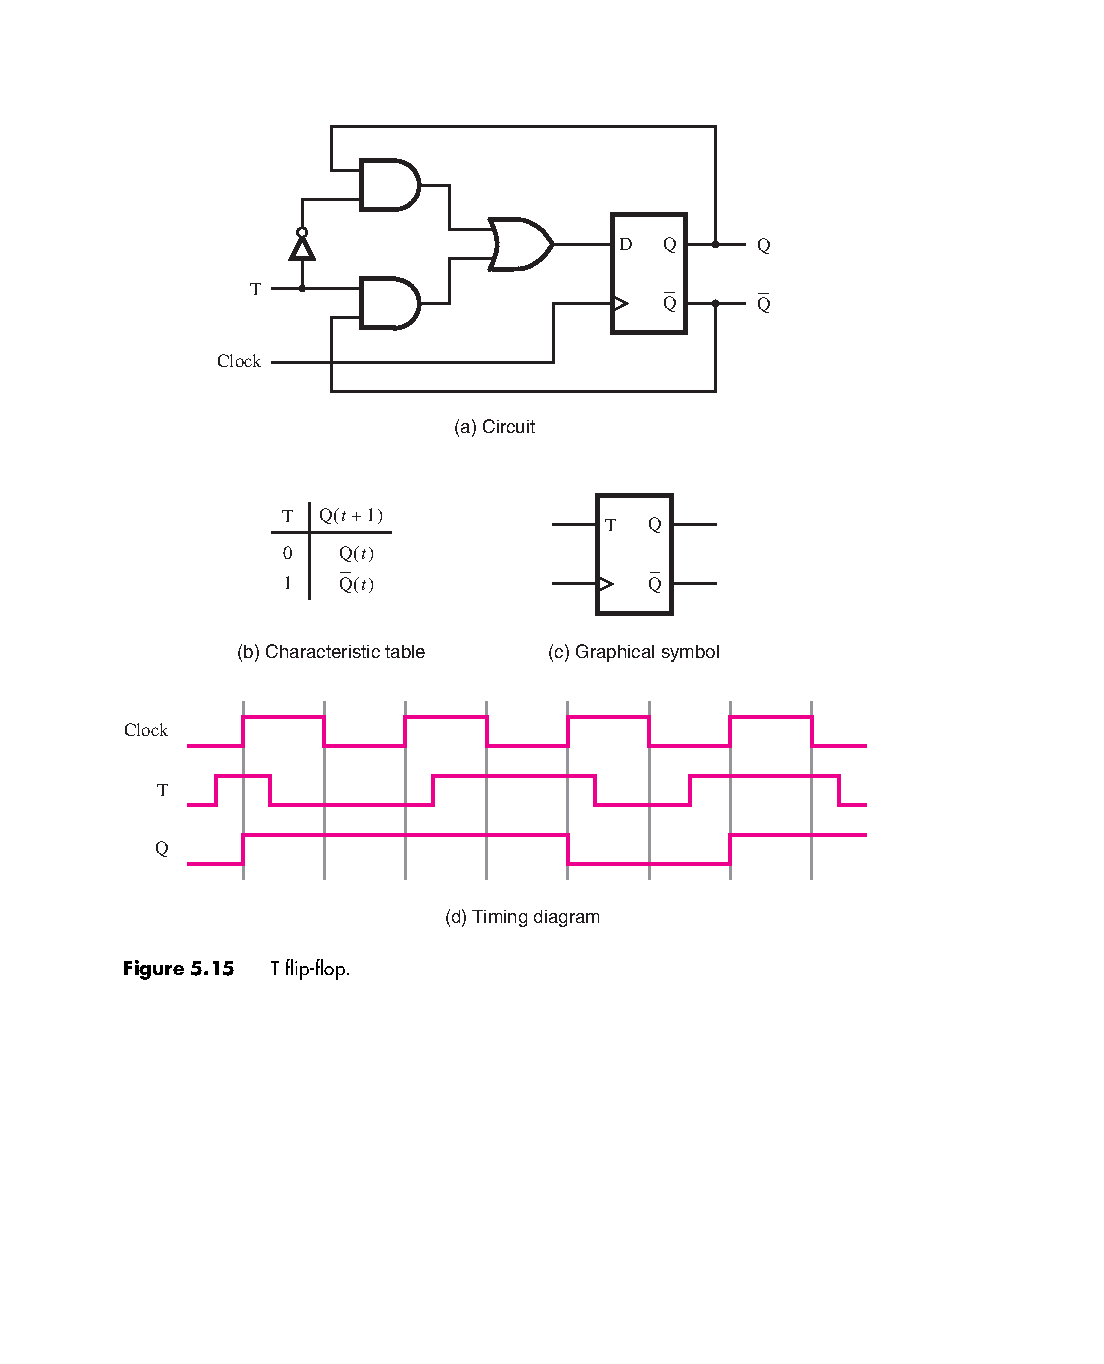
\includegraphics[width=.48\textwidth]{VerilogFig5_15} \\
\end{frame}

\begin{frame}{Flip-flop JK}   \centering
    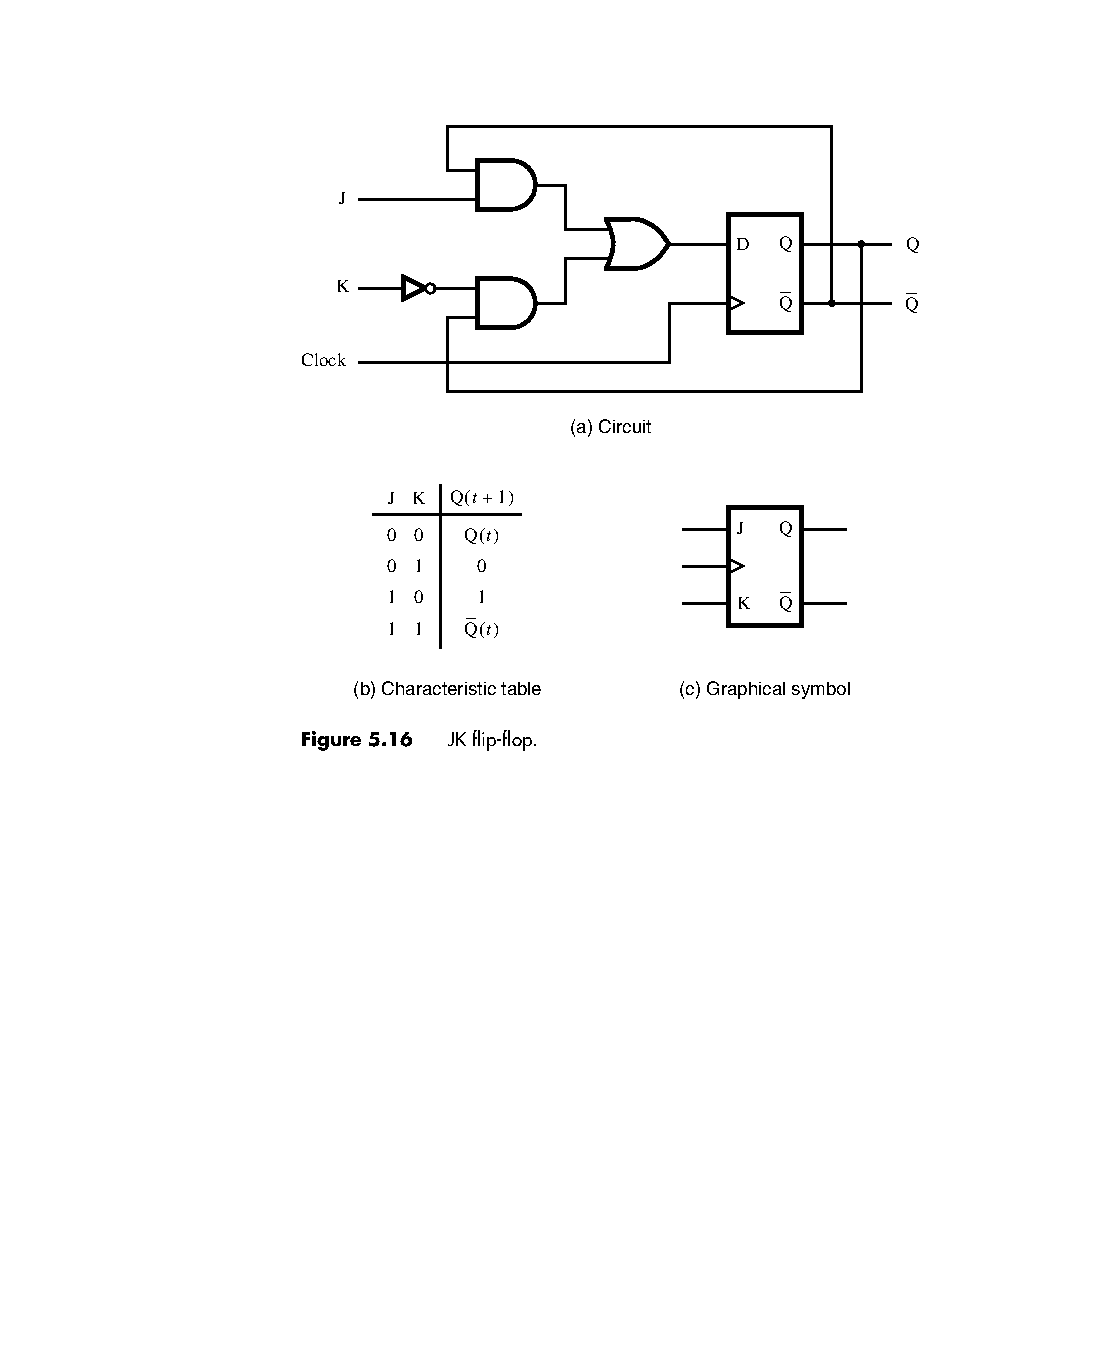
\includegraphics[width=.65\textwidth]{VerilogFig5_16} \\
\end{frame}

\begin{frame}{Bibliografia} 
	\begin{itemize}
		\item \href{https://www.google.com.br/search?q=filetype\%3Apdf+Fundamentals+of+Digital+Logic+with+Verilog+Design+&oq=filetype\%3Apdf}{Brown, S. \& Vranesic, Z. - Fundamentals of Digital Logic with Verilog Design, 3rd Ed., Mc Graw Hill, 2009}
		\item \href{https://www.falstad.com/circuit/e-nandff.html}{https://www.falstad.com/circuit/e-nandff.html}
	\end{itemize}
\end{frame}

\begin{frame}
	\titlepage
\end{frame} 

\end{document}